% !TEX TS-program = XeLaTeX
%\documentclass[oneside]{thesis}
%برای پایان‌نامه ارشد، از خط زیر به جای خط بالا استفاده کنید
\documentclass[Project,oneside]{thesis}
%اگر نسخه دو رو از پایان‌نامه را می‌خواهید، oneside راحذف کنید



\usepackage[colorlinks=true]{hyperref}

\usepackage{longtable}
\usepackage{float}

\usepackage[final]{pdfpages}
\usepackage{array}
\usepackage{multicol}
\usepackage{amssymb}
\usepackage{xepersian}
\usepackage{syntax}
\usepackage{booktabs}





\hypersetup{ 
colorlinks=true,linkcolor=black, anchorcolor=green, citecolor=magenta, urlcolor=cyan, filecolor=magenta, pdftoolbar=true, pdfpagemode=UseOutlines,
}
\settextfont[Scale=1]{XBNiloofar}
\setdigitfont{PGaramond}

\localisecommands
\شروع{نوشتار}

\آرم{\درج‌تصویر{logo}}
\تاریخ{۳ بهمن ۱۳۹۵}
\عنوان{معماری نرم‌افزار پیام‌رسان}
\نویسنده{علی محبی،مهدی کشانی}
\دانشگاه{دانشگاه صنعتی شریف\\دانشکده مهندسی کامپیوتر}
\موضوع{‌ پروژه‌ی معماری نرم‌افزار}

\frontmatter \makethesistitle \pagestyle{empty} \baselineskip1.2\baselineskip



\pagestyle{plain}\pagenumbering{tartibi}\tableofcontents\listoffigures

\mainmatter \pagestyle{headings} \baselineskip1.1\baselineskip
%%%%%%%%%%%%%%%%%%%%%%%%%%%%%%%%%%%%%%%%%%%%%%%%

\chapter{گام اول}\label{chap:1}

\قسمت{مقدمه}
در این گام به معرفی چالش های موجود در یک سامانه‌ی پیام‌رسان می‌پردازیم و سپس راهکارهای موجود را بیان می‌کنیم. این راهکار‌ها می‌توانند جزییات فراوانی داشته باشند که به توضیح آن‌ها در سطح معماری اکتفا می‌کنیم.
\قسمت{تصمیمات معماری}
\زیرقسمت{چهارچوب معماری مورد نیاز سامانه پیام‌رسان}
برای ساخت یک سامانه با نیازمندی‌های گفته شده در ابعاد مورد نظر نیازمند آن هستیم که یک معماری کلی در نظر گرفته شود تا از نظر کارایی و امنیت مناسب باشد.

\زیرقسمت{معماری توزیع شده}
معماری‌ که امروزه در سیستم‌ شبکه های اجتماعی مورد استفاده قرار می‌گیرد به صورت توزیع‌شده\پانویس{distributes architecture}  می‌باشد. پردازش توزیع‌شده رشته‌ای از علوم کامپیوتر می‌باشد که سیستم‌های توزیع‌شده را مورد مطالعه قرار می‌دهد. یک سیستم توزیع‌شده مدلی است که در آن اجزاء بر روی کامپیوتر‌های شبکه شده و این اجزاء از طریق تبادل پیام ارتباط بر قرار می‌کنند و هماهنگ می‌شوند. این اجزا به منظور دستیابی به یک هدف مشترک با یکدیگر تعامل می‌کنند( در اینجا هدف پیاده‌سازی شبکه اجتماعی پیام‌رسان است).  سه ویژگی مهم در سیستم‌های توزیع‌شده عبارتند از : همزمانی اجزاء، نبود clock سراسری و شکست مستقل اجزاء. مثال‌های این سیستم‌ها از SOA based system  \پانویس{Service Oriented Design} تا بازی‌های آنلاین چند نفره (نفرات بسیار بالا) و برنامه‌های peer-to-peer متنوع است. \مرجع{Distri:online}

\subsection{معماری سرویس‌گرا}
همانطور که گفته شد یکی از مثال‌های سیستم‌های توزیع شده SOA ‌ها هستند. زمانی که طراحی یک سیستم مقیاس‌پذیر را در نظر داریم بهتر است وظایف را جدا کنیم و به هر قسمت از سیستم به عنوان یک سرویس نگاه کنیم که دارای واسط به وضوح تعریف شده است. در عمل سیستم‌هایی که اینگونه طراحی می‌شوند گفته می‌شود که دارای معماری سرویس گرا \پانویس{SOA Application program interface} هستند. در این سیستم‌ها هر سرویس دارای زمینه‌ی کاری مجزایی است و تعامل با هر چیزی خارج از آن زمینه از طریق یک واسط انتزاعی انجام می‌شود، به طور کلی از طریق public-facing API\پانویس{Application program interface}.  \مرجع{TheArchi85:online} \\
راهکارهایی که در ادامه معرفی می شوند به راحتی در این چهارچوب معماری می‌توانند گنجانده شوند.

\subsection{انتخاب پروتکل ارتباطی}

پروتکل‌های ارتباطی فراوانی برای ارتباط در اینترنت موجود می‌باشد \متن‌لاتین{(HTTP, HTTPS, TCP, UDP) } پروتکل ارتباطی که مورد استفاده قرار می‌گیرد باید متناسب با نیازمندی‌های عملکردی  \پانویس{Functional Requirements}باشد تا بتوان انتظارات ما را در زمینه کارایی و امنیت برقرار کند.\\
دو نیازمندی عملکردی که دارای ویژگی‌های خاصی می‌باشند عبارتند از امکان مکالمه متنی دونفری و گروهی، مکالمه صوتی و تصویری. پروتکل پیشنهادی برای سامانه مورد نظر پروتکل XMPP  \پانویس{Extensible Messaging and Presence Protocol} می‌باشد. پروتکلXMPP  یک پروتکل خاص منظوره می‌باشد که از مزایای استفاده از این پروتکل می‌توان به موارد زیر اشاره کرد: \مرجع{ChatServ:online} 



\begin{itemize}
\فقره پشتیبانی از پیام‌های ۱:۱ ، چت گروهی، پیام‌های offline
\فقره مکانیزم توکار حظور. کاربر می‌تواند از آنلاین بودن دوستان خود آگاه شود
\فقره توصیفات باز برای شفافیت و حسابرسی
\فقره مدل امنیتی اثبات شده
\فقره مدل قابل گسترش
\فقره دسترسی به پروژه‌های کد باز
\end{itemize}

همانطور که گفته شد این پروتکل قابلیت گسترش دارد. یک نسخه‌ی گسترش یافته Jingle XMPP می‌باشد که تکنولوژی VOIP \پانویس{Voice Over IP}را پشتیبانی می‌کند و از این پروتکل می‌توان برای مکالمه‌های صوتی و تصویری استفاده نمود. \مرجع{Jingle:online}

\زیرقسمت{استفاده از پردازش ابری در شبکه‌های اجتماعی}

امروزه شبکه‌های اجتماعی با قرار دادن امکان اشتراک‌گذاری اطلاعات و برقراری ارتباط بین کاربران، تاثیر فراوانی بر روابط دنیای واقع دارند. لذا این حجم انبوه از کاربران و روابط آن‌ها به تولید حجم عظیمی از اطلاعات می‌انجامد که در پی آن افزایش شدید محاسبات را نیز شاهد هستیم. با یک حساب سرانگشتی خواهیم دید که این اطلاعات و محاسبات بر روی آن‌ها که حتی خود باعث تولید اطلاعات و محاسبات بیشتر نیز خواهند شد، نیازمند ذخیره‌سازی و محاسبات بسیار زیادی هستند. حال در نظر بگیرید که شبکه پیام‌رسان مورد بحث ما علاوه بر این‌ها، کاربران و حتی شرکت‌ها و موسسات را مقدور می سازد تا ربات‌‌های مورد نیاز خود را راه‌‌اندازی کنند. چگونه باید با چالش‌هایی که چنین پردازش‌هایی بر روی کارایی و امنیت سامانه دارند مواجه شویم؟ در اینجا با استفاده از مطالبِ مقاله کنفرانسی \مرجع{Chard} به این سوال پاسخ خواهیم داد. \\
بسیاری ازشرکت‌ها با انگیزه‌ی کاهش هزینه‌ی محاسباتی در نرم‌افزار، سخت‌افزار و تلاش انسانی به سمت استفاده از سرویس‌های ابری رفته‌اند. همچنین شبکه‌های اجتماعی با رشد بسیار زیادی که دارند، با میلیون‌ها کاربر اینترنتی که از طریق وب سایت‌های اینترنتی مختلف در حال مشارکت هستند، در زمانی که حتی شرکت‌ها نیز خود در حال استفاده از شبکه‌های‌ اجتماعی با هدف رشد کسب‌وکار و دسترسی به مشتری‌هایشان هستند به جرگه‌ی ارائه‌دهندگان سرویس‌های ابری پیوسته‌اند. به طور مثال شبکه اجتماعی فیسبوک این امکان را برای کاربران خود مهیا ساخته است؛ که کاربر در سرویس ابری ثبت نام کرده و دوستان می‌توانند به تهیه و استفاده از این منابع از طریق برنامه‌کاربردی فیسبوک\پانویس{Social Cloud Facebook Application}  بپردازند. معماری این ابرِ اجتماعی را در شکل \رجوع{fig:social-cloud} مشاهده می‌کنید.


\begin{figure}[H]
\centering
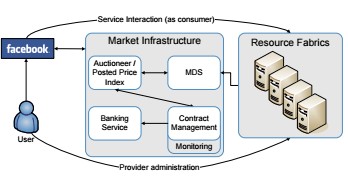
\includegraphics[scale=1]{img/social-cloud.png}
\شرح{مربوط به مقاله کنفرانسی \مرجع{Chard}}
\label{fig:social-cloud}
\end{figure}

\section{رویکردهای مربوط به کارای}
\subsection{بار پردازشی و ترافیکی کلاینت}
برنامه‌های پیام‌رسان در سمت کلاینت از آنجا که معمولاً بر روی گوشی یا تبلت نصب می‌شوند دارای محدودیت‌هایی می‌باشند. از جمله‌ی این محدودیت‌ها می‌توان به کمبود سرعت اینترنت و عملیات های پردازشی اشاره کرد.\\
یک راهکار برای مقابله با این محدودیت‌ها بهینه سازی طراحی واسط کاربری می باشد. واسط‌های‌کاربری دارای اجزای گرافیکی هستند که نمایش آن‌ها نیازمند پردازش و یا دریافت اطلاعات از شبکه هستند. با طراحی مناسب این اجزا می‌توان کارایی را افزایش داد. یکی از روش‌های ساخت واسط‌کاربری با کارایی بالا روش \متن‌لاتین{ Flat Design } می‌باشد، که در نسخه‌های اخیر ویندوز و اینستاگرام از این روش استفاده شده است. این روش تأثیر به‌سزایی در زیبایی برنامه دارد و به طور قابل ملاحظه‌ای کارایی را افزایش می‌دهد.

\subsection{اضافه بار سرور‌ها}
در بسیاری از مواقع درخواست های ورودی به سرور در یک بازه ی زمانی کوتاه بیش از توانایی پاسخگویی سرور می  باشد اما به طور میانگین تعداد درخواست ها متناسب با تعداد نمونه‌های سرویس مورد نظر می باشد. به همین علت نیارمند آن هستیم که درخواست ها نگه داشته شود تا در آینده نزدیک به آن‌ها پاسخ داده شود.\\
یک سیستم صف‌بندی می‌تواند مانع از اضافه بار سرور‌ها شود. در گذشته سامانه‌ی Twitter به این مشکل دچار می‌شد چراکه از هیچ لایه‌ی میانی برای صف‌بندی استفاده نمی‌کرد. لایه میانی در ابتدا توسط یکی از توسعه‌دهندگان Twitter به نام Starling  با زبان \متن‌لاتین{Ruby on Rails} پیاده‌سازی شد. اما مشخص شد که عمل‌کرد  این پیاده‌سازی کند است و دارای Crash Recovery نامطلوبی می‌باشد. سپس چندین زبان دیگر را نیز مورد آزمایش قرار گرفت و در نهایت راه حل توسط یکی از مهندسین نرم‌افزار Twitter به نام Kestrel یافت شد. Kestrel کدهای starling را به زبان Scala باز‌نویسی کرد.\مرجع{Designin77:online}  
\subsection{افزایش بهره وری منابع}

استفاده بهینه از منابع منجر به افزایش کارایی می شود. بدین منظور استفاده از تمام ظرفیت منابع ضروری می‌باشد. یکی از منابع مهم در سیستم‌های کامپیوتری پردازشگر می‌باشد. با استفاده از روش‌های مناسب برنامه‌نویسی و ساختار دهی می‌توان بهره وری لازم در استفاده از پردازشگر‌ها را بدست آورد.\\
یکی از تکنیک‌های مناسب در برنامه‌نویسی چند‌نخی \پانویس{ Multi Threading  } می‌باشد. این تکنیک به مقدار کافی شناخته‌شده می‌باشد. نکته حائز اهمیت این است که زبان برنامه‌نویسی مورد استفاده باید این تکنیک را به درستی پیاده‌سازی کند. یکی از مزیت‌های مهم این تکنیک قابلیت اجرا شدن نخ‌ها بر روی پردازشگر‌های مختلف می‌باشد. برخی از زبان‌های برنامه‌نویسی تنها این قابلیت را با استفاده از \متن‌لاتین{ Time Sharing } شبیه‌سازی می‌کنند.  نمونه‌ای از این زبان‌ها Ruby می‌باشد که از دلایل تغییر قسمت‌هایی از Twitter از این زبان به Scala هم، همین موضوع می‌باشد. \مرجع{Twitter:online} \\
روش دیگر استفاده‌ از الگوی \متن‌لاتین{ Pipes and Filter  } یک وظیفه که پردازش پیچیده‌ای را انجام می‌دهد به دنباله‌ای از عناصر گسسته تجزیه می‌شود که این عناصر می‌توانند به طور مجدد استفاده شوند. این الگو می‌تواند کارایی، مقیاس‌پذیری و قابلیت استفاده مجدد را افزایش دهد. به این صورت که اجازه می‌دهد عناصر وظیفه‌مندی که پردازش انجام می‌دهند به صورت مستقل و مقیاس‌پذیر استقرار یابند. \مرجع{CloudDes:online}

\begin{figure}[H]
\centering
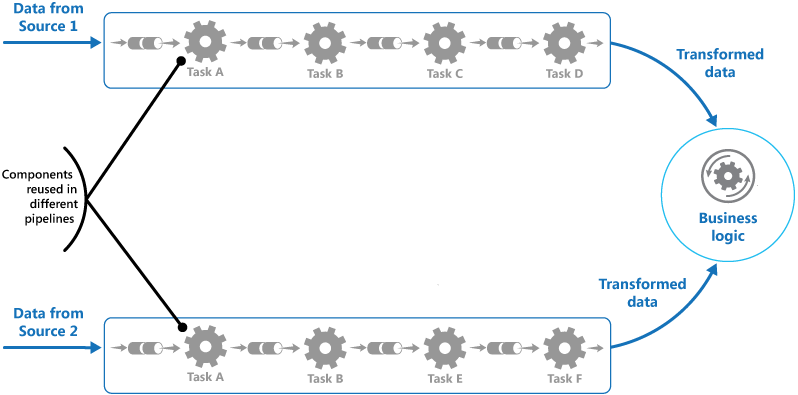
\includegraphics[scale=.4]{img/pipe-filter.png}
\شرح{الگوی \lr{Pipe and Filter}}

\end{figure}

\subsection{مدیریت مناسب داده‌ها}

در یک سامانه‌ی پیام‌رسان انواع مختلفی از داده‌ها موجود می‌باشد از جمله: اطلاعات کاربران، پیام‌های متنی، پیام‌های صوتی، پیام‌های تصویری و غیره. هر نوع از داده‌ها نیازمند نوع خاصی از مدیریت و ذخیره سازی می‌باشد. پایگاه داده‌ای که این اطلاعات را ذخیره می‌کند باید متناسب با این نیازمندی‌ها باشد.\\
انواع مختلفی از پایگاه‌داده‌ها موجود می‌باشد. تعدادی از مدل‌های پایگاه‌داده عبارتند از : سلسله‌مراتبی، شبکه‌ای، گرافی، رابطه‌ای، اسنادی. در هنگام انتخاب پایگاه‌داده باید به این نکته دقت شود که پایگاه‌ داده با چه هدفی مورد استفاده قرار می‌گیرد و با توجه به آن مدل مناسب انتخاب شود. دو مدل پر کاربرد پایگاه‌های‌داده مدل رابطه‌ای و اسنادی می‌باشد. به طور کلی برای ذخیره اطلاعات کاربران از پایگاه‌داده‌های رابطه‌ای و برای ذخیره اشیاء بزرگ و چند رسانه‌ای از پایگاه‌داده‌های NoSQL (به پایگاه داده‌های غیر رابطه‌ای اطلاق می‌گردد) استفاده می‌شود.

\subsection{مدیریت داده های آماری}
در سامانه‌های شبکه های اجتماعی داده‌های موجود می‌باشند که به تنهایی دارای ارزش چندانی نمی باشند و ذخیره‌سازی آن‌ها فضا و سربار پردازشی فراوانی را به وجود می‌آورند اما اطلاعاتی که از مجموعه‌ی این داده‌ها استخراج می‌گردد ارزشمند هستند. در سامانه‌ی پیام‌رسان نمونه‌ای از این داده‌ها رای دادن به محتوای ارسال شده است.\\ 
برای مقابله با این چالش می‌توان از تکنیک aggregation استفاده نمود. تجمع داده‌ها \پانویس{data aggregation}فرآیندی است که در آن داده‌های خام جمع‌آوری می‌شوند و به شکل خلاصه به منظور تحلیل آماری مورد استفاده قرار می‌گیرند. به عنوان مثال داده‌های خام می‌توانند در طول دروه‌های متناوب زمانی جمع‌آوری شوند و داده‌های آماری را مانند مجموع، کمینه، بیشینه، تعداد و میانگین را تهیه شوند. دو نوع تجمع وجود دارد : تجمع زمانی، تجمع فضایی.\مرجع{IBMKnowl:online}
\subsection{افزایش سرعت دسترسی به داده‌ها}
یکی از چالش‌های موجود در سیستم‌ها دسترسی به داده‌ها می‌باشد. همانطور که می‌دانیم مخازن ذخیره‌سازی داده که بر روی دیسک‌های سخت، داده‌ها را ذخیره می‌کنند از سرعت پایین‌تری در برابر سایر قسمت‌ها برخوردار هستند.\\
طبق اصل محلی بودن زمانی، داده‌ای که به تازگی مورد دسترسی قرار گرفته است در آینده‌ی نزدیک هم دوباره مورد دسترسی قرار می‌گیرد. از این جهت می‌توان قسمتی از داده‌ها را بر روی حافظه قرار دهیم که از سرعت دسترسی بالاتری نسبت به دیسک‌های سخت دارند. برای پیاده‌سازی کش می‌توان از پایگاه‌داده‌هایی که بر روی حافظه قرار می‌گیرند استفاده کرد. \\
راهکار دیگر استفاده از الگوی\متن‌لاتین{ Index Table }است. در این الگو بر روی فیلدهایی در مخازن داده ایندکس قرار داده می‌شود که به این فیلد‌ها مکرراً بر اساس \متن‌لاتین{ query criteria  } ارجاع می‌شود. این pattern می‌تواند کارایی query‌ها را افزایش دهد. بدین ترتیب که سریع‌تر محل داده در مخازن مشخص شود.\مرجع{CloudDes:online}

\subsection{افزایش بار کاری سرویس‌ها}
سرور‌های سامانه‌ای با این تعداد از کاربران صدها هزار یا حتی میلیون‌ها درخواست همزمان را باید پاسخ دهند. این پاسخ حاوی متن، عکس یا ویدیو صحیح می‌باشد.  پیاده‌سازی یک سرویس ظرفیت محدودی دارد که در تحت شرایطی (مانند بار کاری زیاد) ممکن است منجر به خطای زمان اجرا ، شکست و یا کاهش کارایی شود.\\
 برای حل این مشکل استقرار اضافی \پانویس{ Redundant deployments } سرویس به وجود می‌آید و یک سیستم متعادل کننده بار \پانویس{Load Balancing} اضافه می‌شود. این سیستم بار کاری را بین پیاده‌سازی‌های سرویس توزیع می‌کند. هدف از الگوی Load Balancing استفاده بهینه از منابع، بیشینه کردن throughput ، کمینه کردن زمان پاسخ و جلوگیری از اضافه بار بر روی یک منبع می‌باشد. اگر یک سرور خراب شود \متن‌لاتین{ Load Balancer } ترافیک را به سایر سرور‌ها هدایت می‌کند و زمانی که سرور جدید افزوده شود به صورت خودکار درخواست‌ها را به آن می فرستد. بدین ترتیب \متن‌لاتین{ Load Balancer } وظایف زیر را بر عهده دارد.\مرجع{Load:online}
 \begin{itemize}
\فقره توزیع درخواست‌های کاربران یا بار شبکه به صورت کارآمد در بین سرور‌ها
\فقره  تضمین دسترس‌پذیری و اعتماد با فرستادن درخواست‌ها به سرور‌هایی که بر خط هستند
\فقره  به وجود آوردن انعطاف‌پذیری در افزودن یا کاستن سرور‌ها در صورت نیاز
 \end{itemize}
 
 \begin{figure}[H]
 \centering
 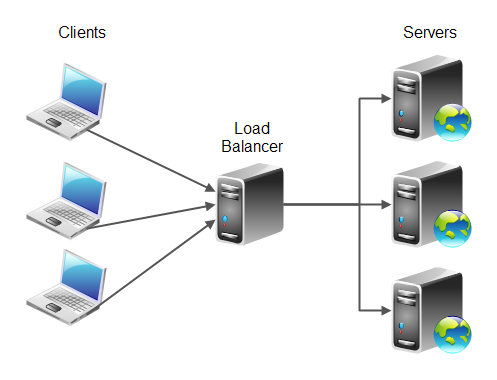
\includegraphics[scale=.6]{img/load-balancer.png}
 \شرح{الگوی \lr{Load Balancer}}
 \end{figure}
 
 
 \subsection{ذخیره‌سازی داده‌ها در مقیاس بالا}
 ذخیره داده‌ها بر روی یک سرور ممکن است موجب محدودیت‌های زیر شود:
 \begin{itemize}
\فقره فضای ذخیره سازی : ذخیره داده‌ها برای یک سامانه‌ی پیام رسان در مقیاس بالا دارای حجم زیادی از داده‌ها می‌باشد که در طول زمان به طور قابل ملاحظه‌ای افزایش می‌یابد. یک سرور معمولاً مقدار محدودی دیسک ذخیره‌سازی فراهم می‌کند.
\فقره منابع محاسباتی: یک سامانه از تعداد زیادی کاربر به صورت همزمان پشتیبانی می‌کندکه هر کدام پرس‌و‌جو‌هایی را اجرا می‌کنند که داده‌هایی را از مخزن داده بازیابی می‌کند. یک سرور ممکن است قدرت محاسباتی لازم برای پشتیبانی از این حجم از بار را نداشته باشد.
\فقره پهنای باند: کارایی مخزن ذخیره‌سازی به وسیله نرخ درخواست‌هایی که دریافت می‌کند و پاسخ‌هایی که می‌فرستد محدود می‌شود.
\فقره جغرافیا: ممکن است لازم باشد داده‌ی تولید شده توسط یک کاربر به دلایل قانونی، انطباق و یا کارایی  در همان منطقه که کاربر قرار دارد ذخیره شود.

 \end{itemize}
 
 برای رفع محدودیت گفته شده می‌توان از الگوی sharding استفاده کرد. این الگو محل ذخیره داده را به یک مجموعه از قسمت‌های افقی یا shard تقسیم می‌کند. هر shard دارای scheme یکسان است اما زیر مجموعه‌ای مجزایی از داده‌ها را نگه‌داری می‌کند. مزایای استفاده از این الگو عبارتند از\مرجع{Sharding:online}: 
 \begin{itemize}
\فقره  مقیاس‌پذیری
\فقره استفاده از کالاهای سخت افزاری از پیش ساخته شده \پانویس{Off the shelf}
\فقره کاهش انتزاع و افزایش کارایی با توزیع متوازن بار کاری
 \end{itemize}
 
 
  \begin{figure}[H]
  \centering
  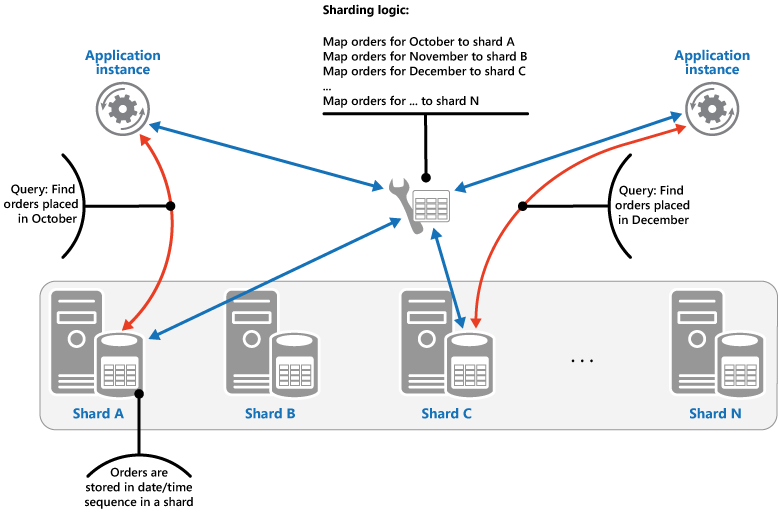
\includegraphics[scale=.4]{img/sharding.png}
  \شرح{الگوی \lr{sharding}}
  \end{figure}
  
 
 
 \subsection{ملاحظات مربوط به مرورگر سمت کلاینت}
 در شبکه‌های اجتماعی به غیر از مسائلی که در سمت سرور داریم، با چالش‌هایی نیز در سمت کلاینت‌ها روبرو هستیم. شبکه‌های اجتماعی و پیام‌رسان‌هایی نظیر اینستاگرام، فیسبوک، تویتر، تلگرام و... علاوه‌ بر اپلیکیشن‌های سمت کلاینتِ خود، این امکان را به کاربران می‌دهند که از طریق مرورگرهای وب نیز به حساب شخصی شبکه‌اجتماعی‌شان متصل شوند. در اینجا راهنماهایی جهت افزایش کارایی در مرورگرهای وب ارائه داده‌ایم که با انجام آن‌ها به دو طریق می‌توان کارایی را افزایش داد؛ اول اینکه دیدی که کاربر نسبت به کارایی سیستم دارد را بهینه سازیم که به آن کارایی درکی \پانویس{Perceived performance} می‌گویند و دوم اینکه به افزایش سرعت واقعی \پانویس{Actual performance} سامانه بپردازیم. \\
 رهنمودهای طراحی زیر که از \مرجع{chapter349:online} آورده شده است به ما کمک می‌کند که کارایی مرورگرهای سمت کلاینت را از دو منظر گفته‌شده افزایش دهیم. این رهنمودها صرفا مربوط به استفاده در شبکه‌های اجتماعی یا پیام‌رسان نیستند و قابل استفاده برای پیاده‌سازی هر نوع برنامه‌ی کاربردی که بر روی مرورگرها پیاده می‌شود هستند.
 \subsubsection{پیاده‌سازی اعتبارسنجی سمت کلاینت }
 
یکی از مسائلی که با آن روبرو هستیم اطمینان از صحت اطلاعات دریافتی از کاربران است. به طور مثال اگر فیلدی قرار است توسط کاربر پر شود، بعضا بایستی مورد بررسی قرار گیرد که آیا نوع داده ‌وارد‌شده یا بازه‌ی وارد شده صحیح است یا نه، به چنین عملیاتی اعتبارسنجی می‌گویند. حال اگر به این عملیات از منظر اینکه چگونه می‌تواند کارایی سیستم را تحت تاثیر قرار دهد نگاه کنیم متوجه چالش‌هایی بر سر راه کارایی می‌شویم که در زیر به ارائه راهکار برای آن می‌پردازیم.\\
اعتبارسنجی را بایستی سمت کلاینت انجام داد تا از ارسال داده‌های نامعتبر به سرور جلوگیری شود، و رفت‌وبرگشت بی‌مورد اطلاعات غیرضروری به حداقل مقدار خود برسد. در عین حال لازم است که به دلایل امنیتی علاوه بر اعتبارسنجی سمت کلاینت، داده‌ها را سمت سرور نیز اعتبارسنجی نماییم زیرا اعتبارسنجی سمت کلاینت به راحتی می‌تواند کنارگذاشته شود.
\subsubsection{نمایش نوار پیشرفت برای عملیات‌های طولانی}
یکی از مواردی که ممکن است با آن مواجه شویم نارضایتی کاربران از سرعت سامانه‌ است. این نارضایتی ممکن است ناشی از یک عملیات طولانی اجتناب‌ناپذیر باشد که راهی نیز برای افزایش سرعت یا مخفی کردن آن از کاربر نیست، در چنین مواردی چه باید کرد تا رضایت کاربران را بازگرداند؟\\
وقتی عملیات طولانی‌ای داریم که قابل صرف نظر کردن نیست و لزوما بایستی اجرا شود خوب است یک نوار پیشرفت سمت کلاینت برای آن عملیات پیاده‌سازی کنیم تا کاربر از زمان باقی‌مانده از عملیات آگاه شود. این کار ممکن است سرعت واقعی سیستم را افزایش ندهد ولی بر روی کارایی ادراکی کاربر تاثیرگذار است. بدین صورت که کاربر با دیدن نوار پیشرفت عملیات، اولا؛ درمی‌یابد که سیستم قفل نشده و در حال پاسخ دادن به درخواست اوست، دوما؛ نسبت به حجم عملیات آگاه می‌شود و در هر لحظه درکی نسبت به مرحله‌ای که در آن است، مقدار سپری‌شده و مقدار باقی مانده پیدا ‌می‌کند و سوما، عملیات به نظر او سریع‌تر می‌آید.

\subsubsection{خودداری از تولید صفحات پیچیده}
گاهی ممکن است در طراحی صفحه وب در سمت کاربر با مشکل سنگین شدن صفحات مواجه شویم که مسلما بر سر راه کارایی سیستم مشکلاتی را به وجود می‌آورد. در مواجهه با این مشکلات و با توجه به محدودیت‌های مختلفی که در این میان به سبب بستر شبکه بین سرور و مشتریان، و تعداد بالای مشتریان یک شبکه اجتماعی به‌وجود می‌آید به چه نکاتی می‌بایست توجه کرد و چه راهکاری می‌بایست در پیش گرفت؟\\
صفحات پیچیده معمولا شامل فراخوانی‌های حجیم متعدد از سرور هستند که این خود انتقال حجم عظیمی از اطلاعات از طریق شبکه را ایجاب می‌کند. هنگام طراحی صفحات پیچیده و صفحات دارای گرافیک سنگین بایستی محدودیت‌های پهنای باند را در نظر بگیریم و به پراکندگی جغرافیایی مشتریان شبکه اجتماعی خود توجه داشته باشیم. حتی بررسی‌های موشکافانه‌تری می‌توان من باب دسترسی کاربران مختلف به پهناهای باند متفاوت انجام داد و بر روی پیچیدگی صفحات با توجه به نُرم جامعه آماری مشتریان برنامه‌ریزی دقیق‌تری کرد. توجه به این نکته حائز اهمیت است که در تصمیمات معمارانه خیلی اوقات با سبک‌سنگین‌ کردن‌های بسیار اساسی مواجه هستیم لذا در این‌جا بایستی تعادلی مابین پیچیدگی صفحات و جذابیت و قابلیت یادگیری سیستم ایجاد کنیم. چرا که این عوامل نیز خود در جذب مشتریان بسیار مهم هستند.

\subsubsection{بارگذاری تکه‌تکه‌ی خروجی}
راه حل دیگری که برای چالش قبل ارائه می‌شود در زیر آورده شده است: \\
 می‌توان هر بار یک تکه از صفحات وب را بارگذاری کرد. قسمت بالایی یا چپی اکثر صفحات معمولا برای همه‌ی درخواست‌ها مشابه‌ هستند. می‌توان قسمت منحصر به فرد صفحه را پس از اتمام پردازشِ درخواست به جریان انداخت. در همه‌ی این حالات متن‌‌ها می‌توانند قبل از تصاویر به جریان انداخته شوند.
 
\subsubsection{کاهش اندازه‌ و تعداد تصاویر}
 
 سامانه‌ای که ما به آن می‌پردازیم دارای امکان تبلیغ در گروه‌ها می‌باشد که این امر را می‌توان در دو مرحله بررسی کرد. مرحله اول؛ قرار دادن تصاویر مربوط به تبلیغات در کانال‌هاست، که باید بررسی کنیم چه اثراتی بر روی کارایی و امنیت سامانه دارد. مرحله دوم؛ پرداخت هزینه‌ی تبلیغات است که قسمت عمده‌ی این مرحله به دلیل استفاده از سرویس‌های بانک‌ها به انتخاب سرویس مناسب برمی‌گردد. لذا در اینجا تمرکز خود را بر روی مرحله‌ی اول می‌گذاریم، و چالش سنگین شدن صفحات را که سرمنشا آن تصاویر و عکس‌هایی با حجم بالاست را بررسی می‌نماییم. در زیر برای این مشکل راهکاری ارائه شده است. \\
 بایستی از تصاویر کوچک و فشرده‌شده استفاده کنیم و تعداد تصاویر را در حداقل خود نگه‌‌ داریم تا حجم داده‌ای که نیاز است به مرورگر فرستاده شود کاهش یابد. فرمت‌های GIF و JPEG هر دو فشرده هستند، اما فرمت GIF معمولا وقتی تصاویر فشرده‌شده دارای رنگ‌های کمی هستند فایل‌های کوچکتری تولید می‌کند. در حالی که فرمت  JPEG معمولا وقتی تصاویر شامل رنگ‌های زیادی باشند فایل‌های کوچکتری تولید می‌کند.
 
 \section{رویکردهای مربوط به امنیت}
 \subsection{آگاهی از وضعیت سرویس‌ها}
 لازم است که از درستی عملکرد سرویس‌ها آگاهی داشت تا از بروز مشکل و حمله اطلاع پیدا کرد و تدابیر لازم انجام شود. یکی از حملات متداول \متن‌لاتین{Denial Of Service } می‌باشد که از دسترسی کاربران مشروع به سرویس جلوگیری می‌شود. یکی از روش‌های این حمله ایجاد‌های درخواست‌های فراوان می‌باشد که در نتیجه‌ی آن بار سرور افزایش فراوانی خواهد داشت، به صورتی که دیگر پاسخگویی درخواست‌های قانونی نمی‌باشد. از طرف دیگر ممکن است مشکلی در سرویس وجود داشت باشد و درخوست‌ها به درستی پاسخ داده نشوند.\\
 از انواع سیستم‌های نظارتی می‌توان استفاده نمود. از نمونه‌های استفاده شده می‌توان به سیستم‌های نظارت بر ترافیک و سیستم‌های نظارت بر درستی سرویس‌ها نام برد. از این سامانه‌ها می‌توان برای تشخیص مشکلات امنیتی و حملات سایبری استفاده کرد. به عنوان مثال افزایش غیر‌منطقی ترافیک نشان‌دهنده‌ی حمله می‌باشد. و خارج شدن یک سرویس از دسترس می‌تواند نشان‌دهنده‌ی \متن‌لاتین{ Denial of Service  } باشد.\مرجع{CloudDes:online}
 
  
\begin{figure}[H]
\centering
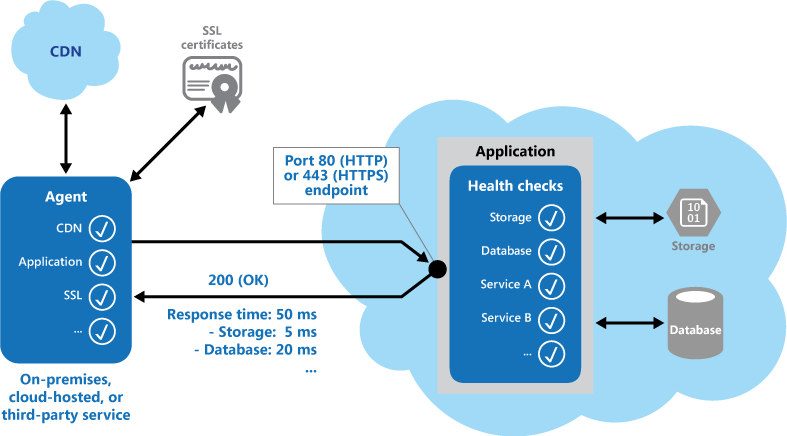
\includegraphics[scale=.4]{img/monitoring.png}
   \شرح{الگوی \lr{monitoring}}
\end{figure}

\subsection{تهیه نسخه‌ی پشتیبان از داده‌ها}
  
 به دو دلیل لازم است از داده‌ها نسخه‌ی پشتیبان تهیه شود. یکی به منظور افزایش امنیت و دیگری کارایی.در واقع می‌بایست در صورتی که به علت مشکل یا حمله، داده‌ها دچار نقصان شوند بتوان آن‌ها را ترمیم کرد. همچنین دیسک‌های سخت دارای محدودیت‌هایی هستند که در کارایی تأثیر گذارند. با وجود چندین نسخه از داده‌ها، از این محدودیت‌ها کاسته می‌شود. فرآیند تهیه پشتیبان باید به صورت خودکار و با مدیریت مناسب انجام گیرد.
 تکنولوژی RAID  \پانویس{redundant array of inexpensive disks } یک تکنولوژی مجازی‌سازی ذخیره‌سازی داده می‌باشد که در آن چند دیسک فیزیکی با هم ترکیب می‌شوند و یک واحد منطقی را به منظور تکرار داده یا بهبود کارایی به وجود می‌آورند. این تکنیک دارای سطوح مختلفی می‌باشد و سطوح بالاتر دارای تدابیر امنیتی بیشتری می‌باشند. \مرجع{RAIDWiki:online}
 
\subsection{رعایت نکات امنیتی} 
 در پیاده‌سازی سامانه‌های نرم‌افزاری که مورد استفاده‌ی کاربران متعددی می‌باشند، لازم است نکاتی را در راستای ارتقای امنیت رعایت نمود. بدین منظور رهنمودهایی1 در جدول  \رجوع{tab:guid}  فراهم شده است، که در یک ستون دسته‌ای از رهنمودها و در ستون دیگر خلاصه‌ای از آن دسته رهنمود قرار می‌گیرد. به دلیل نبود کلمات فارسی معادل و کاهش انتقال مفهوم از ترجمه آن‌ها خودداری شده است. \مرجع{chapter349:online}
 
\begin{table}[H] 
        \centering \caption{رهنمودهای امنیتی}
        \label{tab:guid}
        \renewcommand*{\arraystretch}{2}
 \begin{latin}


 \begin{tabular}{ p{3cm} p{11cm} }
            \hline
  
			\bf Category & \bf Guidelines\\
            \hline
 			 Input Validation & Do not trust input; consider centralized input validation. Do not rely on client-side validation. Be careful with canonicalization issues. Constrain, reject, and sanitize input. Validate for type, length, format, and range.\\
 			 
 			 Authentication & Partition site by anonymous, identified, and authenticated area. Use strong passwords. Support password expiration periods and account disablement. Do not store credentials (use one-way hashes with salt). Encrypt communication channels to protect authentication tokens. Pass Forms authentication cookies only over HTTPS connections.\\
 			 Authorization & Use least privileged accounts. Consider authorization granularity. Enforce separation of privileges. Restrict user access to system-level resources.\\
 			 Configuration Management & Use least privileged process and service accounts. Do not store credentials in plaintext. Use strong authentication and authorization on administration interfaces. Do not use the LSA. Secure the communication channel for remote administration. Avoid storing sensitive data in the Web space.\\
 			 Sensitive Data & Avoid storing secrets. Encrypt sensitive data over the wire. Secure the communication channel. Provide strong access controls on sensitive data stores. Do not store sensitive data in persistent cookies. Do not pass sensitive data using the HTTP-GET protocol.\\
 			
        \end{tabular}
         \end{latin}
 \end{table}
 
 
 \begin{table}[H] 
         \centering \caption{رهنمودهای امنیتی(ادامه)}
         \renewcommand*{\arraystretch}{2}
  \begin{latin}
 
 
  \begin{tabular}{ p{3cm} p{11cm} } 
       \hline
    
  			\bf Category & \bf Guidelines\\
              \hline
  Session Management & Limit the session lifetime. Secure the channel. Encrypt the contents of authentication cookies. Protect session state from unauthorized access.\\
  			 Cryptography & Do not develop your own. Use tried and tested platform features. Keep unencrypted data close to the algorithm. Use the right algorithm and key size. Avoid key management (use DPAPI). Cycle your keys periodically. Store keys in a restricted location. \\
              Parameter Manipulation & Encrypt sensitive cookie state. Do not trust fields that the client can manipulate (query strings, form fields, cookies, or HTTP headers). Validate all values sent from the client. \\
              Exception Management & Use structured exception handling. Do not reveal sensitive application implementation details. Do not log private data such as passwords. Consider a centralized exception management framework. \\
              Auditing and Logging & Identify malicious behavior. Know what good traffic looks like. Audit and log activity through all of the application tiers. Secure access to log files. Back up and regularly analyze log files. \\
              
\end{tabular}
\end{latin}
\end{table}

\subsection{کاهش سطح آشکار سرویس‌ها}
سرویس‌ها با پذیرش درخواست‌های کاربران عملکرد خود را افشا می‌سازند.\متن‌لاتین{ End point‌}هایی که کاربران به آن متصل می‌شوند شامل کدهایی است که عمل احرازهویت ، پردازش درخواست و دسترسی به مخازن ذخیره‌سازی را انجام می‌دهند. یک کاربر مخرب می‌تواند به داده‌های حساسی دست پیدا کند.\\
الگوی Gatekeeper از یک \متن‌لاتین{ dedicated host}  استفاده می‌کند که به عنوان یک broker بین کاربران، برنامه و سرویس‌ها عمل می‌کند. بدین ترتیب از برنامه و یا سرویس‌ها محافظت می‌شود. درخواست‌ها تأیید و پاک‌سازی می‌شوند و در اجزا سیستم رد و بدل می‌شوند. این الگو لایه اضافی از امنیت را تهیه می‌کند و سطح مورد حمله سیستم را محدود می‌کند.\مرجع{CloudDes:online} 
\begin{figure}[H]
\centering
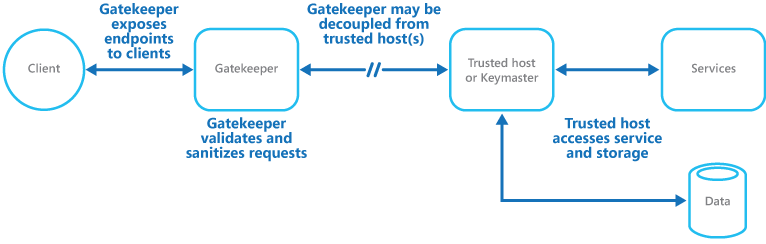
\includegraphics[scale=.6]{img/gatekeeper.png}
   \شرح{الگوی \lr{gatekeeper}}
\end{figure}

\subsection{فایروال}
با توجه به حساسیت اطلاعات و محاسباتی که در سرور شبکه‌های اجتماعی انجام می‌شود، برقراری امنیت در هاست‌ها و سرور‌های مربوطه امری حیاتی است. با در نظر گرفتن حجم بالای اطلاعات و توجه به تعداد زیاد مدیران و کارمندانِ چنین محیطی، این نکته مشخص است که با چالش‌های فراوانی در مسیر برقراری امنیت روبرو خواهیم بود. از جمله اینکه همه‌ی افراد می‌بایست در خصوص امنیت، دانش و تکنیک مناسبی داشته باشند که با توجه به تعداد بالای افراد امری بسیار پرهزینه، ریسکی و حتی می‌توان گفت نشدنی است. برای حل چنین چالشی چاره‌اندیشی فراگیری با نام فایروال صورت گرفته است که ما در اینجا با توجه به مطالبی که در \مرجع{security15:online} آورده شده است به این موضوع خواهیم پرداخت.\\
فایروال سیستمی است که با فیلترکردن ترافیک ورودی و خروجی شبکه، بر مبنای یک سری قوانین تعریف شده توسط کاربر امنیت شبکه را تامین می‌کند. به طور کلی، هدف از یک فایروال کاهش امکان وقوع یا جلوگیری از وقوع ارتباطات ناخواسته‌ی شبکه است، در عین حال که ارتباطات مشروع با آزادی اجازه‌ی وقوع دارند. در بسیاری فراساختارهای سرور، فایروال‌ها یک لایه‌ی ضروری از امنیت را فراهم می‌کنند که با سایر معیارها ترکیب شده است و در برابر دسترسی مخرب حمله‌کنندگان به سرورهای شما جلوگیری می‌کنند.\\
مزیت‌های فایروال:
\begin{itemize}
\فقره می‌توان ترافیک بیش از حد را فیلتر کرد.
\فقره می‌توان یک محدوده IP خاص یا پورت را بلاک کرد به جای تلاش برای مطمئن شدن از اینکه هیچ سرویسی بر روی یک ماشین خاص وجود ندارد که به آن پورت گوش کند. یا می‌توان دسترسی را با استفاده از TCP/Wrappers لغو کرد.
\فقره فایروال‌ها می‌توانند هنگامی که کاربران یا مدیرانی داریم که نسبت به امنیت بی‌توجه‌ یا بی‌اطلاع‌اند، به کمک ما بیایند و یک خط دفاعی دومی برای آن‌ها فراهم کنند. بدون ‌‌آن‌ها همه‌ی افراد می‌بایست به صورت کامل اطمینان حاصل کنند که هاست‌ها امن هستند، که این خود نیازمند درک بالایی از امنیت توسط افراد می‌باشد.
\فقره فایروال‌ها می‌توانند یک تاریخچه‌ی مرکزی برای ما فراهم آورند. به طور مثال می‌توان با استفاده از تاریخچه‌ی فایروال‌ها کاربرانی که سعی در متصل شدن به پورت‌های مشترک همه‌ی سرورهای ما در فواصل معین زمانی دارند را پیدا کرد. برای انجام این‌ کار بدون استفاده‌ از فایروال‌ها یک نفر می‌بایست تاریخچه‌های مختلف را از سرورها یا هاست‌های مختلف ترکیب کند تا یک دید متمرکز به دست آورد.
\end{itemize}

\subsection{تعامل سرویس‌ها}
با استفاده از مطالبی که در  مرجع \مرجع{Messaging:online} در مورد معماری‌ توزیع‌شده و سرویس‌گرا گفته شده است تصمیم گرفتیم به منظور افزایش مقیاس‌پذیری در دل معماری توزیع شده خود یک معماری سرویس‌گرا در نظر بگیریم لذا در این مسیر با چالش‌هایی مواجه هستیم. ارتباط مابین سرویس‌های ما چگونه برقرار می‌شود؟ چگونه بایستی یک پیام بین سرویس‌ها جا‌به‌جا شود؟ نوع این پیام‌ها چیست؟ هر کدام از انواع پیام‌های منتقل شده دارای چه معنایی هستند؟ کانال چیست و چگونه مورد استفاده قرار می‌گیرد؟ پیام‌های یک سرویس چگونه به مقصد می‌رسند؟ و ... . در زیر راهکارهایی برای مواجهه با چالش‌هایی که در راستای ارتباط سرویس‌ها با آن مواجهیم آورده شده است.\\
پیام خود یک نوع داده‌ساختار محسوب می‌شود مانند انواع دیگرِ داده‌ای، از جمله؛ رشته، آرایه، رکورد و یا یک شئ. این نوع می‌تواند به سادگی به عنوان یک داده‌ تفسیر شود، یا به عنوان توصیف یک فرمان که باید در گیرنده به آن رسیدگی شود، و یا به عنوان توصیف یک رویداد که در فرستنده اتفاق افتاده است. فرستنده می‌تواند یک پیام فرمان بفرستد، که مشخص کننده تابع یا متدی در گیرنده باشد که فرستنده قصد ارتباط با آن را دارد. همچنین می‌تواند یک پیغام مستند ارسال کند که فرستنده را برای انتقال یکی از داده‌ساختارهایش به گیرنده فعال کند. یا می‌‌تواند یک پیام رویداد ارسال کند و گیرنده را از تغییری در فرستنده آگاه سازد.\\
کانال‌ها به عنوان یک صف شناخته می‌شوند، و درواقع مسیرهای منطقی برای انتقال پیغام‌ها هستند. یک کانال همانند مجموعه‌ یا آرایه‌هایی از پیام‌ها رفتار می‌کند، در حالی که بین چندین کامپیوتر  به اشتراک گذاشته شده است و می‌تواند به صورت همزمان توسط چندین برنامه مورد استفاده قرار گیرد. البته خود کانال‌ها نیز انواع مختلفی دارند، که در این‌جا مجال ورود به جزئیات آن‌ها نیست. 

\chapter{گام دوم}\label{chap:2}
\section{بررسی ‌الگوهای مولفه اتصال مختلف در سامانه‌ی ما}

\زیرقسمت{الگوی ‌‌Broker}

الگوی ‌‌Broker سخن از این نکته می‌گوید که در سامانه‌هایی که سیستم مجموعه‌ای از سرویس‌های توزیع‌شده است  پیاده‌سازی مشکل خواهد بود و ارتباط  اجزای سیستم و در دسترس بودن سرویس‌های کامپوننت‌های مختلف برای ما مشکل‌ساز خواهد شد. لزوم اطلاع از مکان و نوع سرویس‌ها از سوی  کاربران  برای استفاده از سرویس‌ها باعث ایجاد و تقویت مشکلات ذکر شده خواهد شد. راه حلی که این الگو پیشنهاد میدهد استفاده از یک میانجی است که در مورد سویس‌ها اطلاع دارد و کاربران و سرویس‌دهندگان به جای اتصال به یکدیگر به آن متصل می‌شوند. با توجه به اینکه سامانه ما یک سیستم توزیع شده است که سرویس‌هایی در آن ارائه می‌شود، قاعدتا با مشکلات گفته شده مواجه خواهیم شد لذا راه حلی که این الگو  ارائه داده است  برای سامانه‌ای مشابه سامانه ما مناسب به نظر می‌رسد.



\زیرقسمت{الگوی ‌‌Model-View-Controller}

مسئله‌ای که این الگو به آن توجه کرده است تغییرات مداوم واسط کاربری است، بدین معنا که کاربران اطلاعات مختلف را به اشکال مختلف خواهند دید و با آن تعامل خواهند داشت و لذا بسیار  مفید خواهد بود اگر این واسط در عین اینکه  حالت فعلی اطلاعات را به کاربران نشان می‌دهد عملکردی مستقل از عملکرد کاربردی سیستم داشته باشد. راه حلی که این الگو ارائه داده است تقسیم عملکرد سیستم بین سه مولفه model ، view و controller است. مولفه view وظیفه‌ی نمایش بخش‌هایی از داده و تعامل با کاربران را بر عهده دارد، model شامل داده‌های سامانه می‌شود و controller میانجی بین این دو است و مدیریت اخطارهای تغییر حالت را بر عهده دارد. به طور کلی در شبکه‌های اجتماعی و سامانه‌های پیام‌رسان با توجه به اینکه تعداد کاربران هم بسیار بالا است و سیستم بایستی با کاربران تعامل داشته باشد واسط‌کاربری و تغییرات آن برای ما حیاتی خواهد شد.علاوه بر این جذابیت چنین سامانه‌ای برای جذب کاربران اهمیت دارد لذا اگر امکانات شخصی سازی در  واسط‌کاربری به کاربران داده شود تاثیر خوبی خواهد داشت. با توجه به همه‌ی این نکات الگوی MVC برای سامانه‌ی ما مناسب به نظر می‌رسد.


\قسمت{دیدهای مولفه و اتصال}
\زیرقسمت{مولفه IM}
\زیرزیرقسمت{دید اصلی}
\زیرزیرقسمت{عناصر}
\begin{itemize}

\فقره Server : این مولفه مسؤولیت مقداردهی اولیه و برپایی مولفه‌های connection ، muc و singlchat را برعهده دارد. همچنین با مولفه‌ی بیرونی admin تعامل دارد.
\فقره muc : این مولفه عملیات‌های مربوط به چت گروهی را بر عهده دارد.
\فقره singlechat : چت دو نفره در این مولفه پشتیبانی می‌شود. 
\فقره connection :  انواع مختلفی از ارتباطات با محیط بیرون را سازماندهی می‌کند.
\فقره auth : وظایف مربوط به احراز هویت افراد در این مولفه انجام می‌گیرد.
\فقره roster : فهرست‌های مختلفی را نگهداری می‌کند. مانند فهرست مخاطبین فرد، فهرست افراد یک گروه.
\فقره filetransfer : تبادل فایل به وسیله‌ی این مولفه انجام می‌گیرد. این فایل ها در متن چتها تبادل می‌شود.
\فقره  pubsub : پیاده سازی الگوی publish-subscribe که اطلاع رسانی رویدادها را بر عهده دارد. 
\فقره bot : عملیات‌های مربوط به رباتها در این مولفه قرار دارد.
\فقره ldap : دسترسی به اطلاعات مکان افراد یا اشیاء در این مولفه قرار داد. 
\فقره session : تعامل کاربران با سامانه از طریق این مولفه صورت می‌گیرد.
\فقره media : امور رسانه‌ای مانند عکسهای موجود در حساب کاربری و تماس صوتی یا تصویری در این قسمت قرار می‌گیرد.
\end{itemize}



\زیرقسمت{مولفه database}

\زیرزیرقسمت{دید اصلی}

\زیرزیرقسمت{عناصر}

\begin{itemize}

	

	\فقره schemadata : این مولفه مسؤولیت مدریت شِما و  داده‌ها را دارد و تغییرات و به روز رسانی‌های آن و اطمینان از به روز بودن پایگاه داده نسبت به شما را بر عهده دارد. 

	\فقره bugfix :  این مولفه در مواردی در صورت لزوم به مشکلاتی که رخ می‌دهند رسیدگی می‌کند.

	\فقره connectionmanager :  مدیریت ارتیاظ‌هایی که با پایگاه داده برقرار می‌شود را بر عهده دارد.

	\فقره connectionprovider : وظیفه فراهم‌سازی ارتباط برای مولفه‌های دیگر با دیتابیس را بر عهده دارد.

	

\end{itemize}





\زیرقسمت{مولفه util}

\زیرزیرقسمت{دید اصلی}

\زیرزیرقسمت{عناصر}

\begin{itemize}



\فقره cert : این مولفه مسؤولیت مدریت یک سری اختیارات و گواهی‌های صادر شده از سوی مدیر را به عهده دارد.

\فقره log :  این مولفه تاریخچه‌ی درخواست‌هایی که به حافظه سیستم می‌آید و دسترسی‌هایی که انجام می‌شود را نگه می‌دارد.

\فقره cache : این مولفه داده‌هایی که نیاز است را در خود نگه می‌دارد.

\فقره defaultcache : این مولفه داده‌هایی که در حافظه موجود است را ارائه می‌د‌هد.

\فقره cachefactory : این مولفه داده‌هایی که نیاز است از پایگاه داده می‌گیرد و در حافظه ذخیره می‌کند.

\فقره commons : وظیفه تبادل داده‌ها با پایگاه داده را بر عهده دارد.



\end{itemize}



زیرقسمت{مولفه admin}

\زیرزیرقسمت{دید اصلی}

\زیرزیرقسمت{عناصر}

\begin{itemize}

	

	\فقره adminconsole : یک سری اختیارات خاص در اختیار مدیران قرار می‌دهد مثل دسترسی به پایگاه‌داده و ایجاد یک سری تغییرات.



\end{itemize}





\زیرقسمت{نیازمندی‌های کارکردی}

در این بخش به بیان نیازمندی‌های کل سیستم خواهیم پرداخت. همانطور که در زیر می‌بینید کل سیستم در سطح اول به چندین مولفه تقسیم می‌شود که در زیر برای هر یک از این مولفه‌ها و زیر مولفه‌هایشان نیازمندی‌های کارکردی را بیان می‌کنیم که در مجموع کل نیازمندی‌های کارکردی سیستم را پوشش می‌دهد.
\زیرزیرقسمت{IM}
\begin{itemize}
\فقره ldap : 
\begin{itemize}
\فقره مکان‌یابی افراد
\فقره مکان‌یابی منابع مانند فایلها در شبکه 
\end{itemize}
\فقره   connection :
\begin{itemize}
\فقره  مدیریت ارتباطات ورودی و خروجی
\فقره فراهم آوردن بستر مناسب جهت برقراری ارتباط با انواع پروتکل‌های مناسب
\end{itemize}
\فقره media : 
\begin{itemize}
	\فقره ایجاد تماس صوتی در چت دو تفره
	\فقره ایجاد تماس تصویری در چت دو تفره
	\فقره فراهم سازی و مدیریت تصاویر مربوط به حساب های کاربری
	
\end{itemize}
\فقره  session :
\begin{itemize}
	\فقره سازماندهی ارتباطات کاربران با سرور در حالت نیمه پایدار
	\فقره ارتباط با مولفه های مربوط به چت به منظور فراهم کردن عملکردهای پیام رسان
	\فقره اطلاع از وضعیت کاربران
	\فقره ذخیره‌ی اطلاعات تعاملات
\end{itemize}

\فقره muc : 
\begin{itemize}
\فقره ایجاد گروه به منظور چت گروهی
\فقره ایجاد کانال
\فقره تبادل پیام در گروه و کانال
\فقره مدیریت تبلیغات در کانال‌ها
\فقره دریافت داده از ربات‌ها و انتشار
\فقره ذخیره محتواهای چتها و کانالها
\end{itemize}

\فقره singlechat :

\begin{itemize}
\فقره ایجاد مکالمه جهت چت دو نفره
\فقره تبادل پیام در چت
\فقره دریافت داده از ربات‌ها و انتشار
\فقره ذخیره محتواهای چت 

\end{itemize}
\فقره bot : 
\begin{itemize}
\فقره فراهم ساختن سرویس‌های لازم جهت ساخت ربات
\فقره ارسال دستور به ربات ها
\فقره دریافت و انتشار پاسخ ربات ها
\end{itemize}

\فقره pubsub :
\begin{itemize}
\فقره انتشار وضعیت کاربران ماننذ آنلاین بودن
\فقره انتشار رویدادها
\end{itemize}
\فقره  filetransfer : 
\begin{itemize}
\فقره انتقال فایل در محیط چت دو نفره
\فقره انتقال فایل در محیط گروه و کانال نفره
\end{itemize}
\فقره roster :
\begin{itemize}
\فقره نگهداری لیست مخطبین کاربران
\فقره نگهداری لیست اعضای گروه
\فقره نگهداری لیست اعضای کانال
\end{itemize}

\فقره auth: 
\begin{itemize}
\فقره مدیریت حسابهای کاربری
\فقره ایجاد حساب کاربری جدید
\فقره احراز هویت افراد
\فقره مشخص کردن میزان دسترسی افراد
\end{itemize}
\فقره server :
\begin{itemize}
\فقره مقداردهی و آماده سازی مولفه‌های connection ، muc ، singlechat
\فقره اجرا کردن دستورات admin در رابطه با نحوه‌ی کار پیام رسانی
\end{itemize}
\end{itemize}

\زیرزیرقسمت{database}


\begin{itemize}	

	\فقره schemadata : 

	\begin{itemize}	

		\فقره	مدیریت کردن شِما و پایگاه داده

		\فقره	مدیریت  کردن تغییرات  شِما و پایگاه داده

		\فقره	مدیریت  کردن به روزرسانی‌های شِما و پایگاه داده

		\فقره 	اطمینان حاصل کردن از تطابق پایگاه‌داده با شما 

		\فقره	پاسخ به پرس‌وجوها

		

	\end{itemize}

	\فقره bugfix :

	\begin{itemize}	

		

		\فقره کشف کردن خطاهای مولفه دیتابیس

		\فقره یافتن منشا ارور

	   \فقره نشان دادن واکنش مناسب به خطای مربوطه مثل پیام خطای مناسب و یا تصحیح مناسب

		

	\end{itemize}

	\فقره connectionmanager :

	\begin{itemize}

	   \فقره دریافت کردن درخواست‌های مولفه‌های دیگر برای برقراری ارتیاط با پایگاه‌داده

		\فقره حصول اطمینان از امنیت درخواست‌ها

		\فقره ارسال کردن درخواست‌های مطمئن به پایگاه‌داده

		\فقره ممانعت ا ارسال درخواست‌های مشکوک

		\فقره حفظ ترتیب درخواست‌ها

	\end{itemize}

	

	\فقره connectionprovider : 

	\begin{itemize}

		\فقره ارسال کردن پاسخ‌های مناسب به مولفه‌های مناسب

		\فقره حفظ ترتیب ارسال‌ها

		

	\end{itemize}	

\end{itemize}



\زیرزیرقسمت{util}

\begin{itemize}	

	\فقره cert : 

	\begin{itemize}	

		\فقره	دریافت کردن درخواست‌های مدیر

		\فقره	بررسی کردن درخواست‌های مدیر

	   \فقره	جدا کردن درخواست‌های ایمن و معتبر از غیرایمن و نامعتبر

		\فقره 	ثبت درخواست‌های معتبر در پایگاه داده

		

	\end{itemize}

	\فقره log :

	\begin{itemize}	

		

		\فقره دریافت درخواست‌های حافظه‌ای

		\فقره دریافت پاسخ‌های حافظه‌ای

	   	\فقره ایجاد تاریخچه از روی آن‌ها

		

	\end{itemize}

	\فقره cache :

	\begin{itemize}

	    \فقره دریافت کردن درخواست‌های دسترسی به داده

		\فقره ذخیره داده‌های پراستفاده و محلی

		\فقره پاسخ به درخواست‌های دریافتی

		

	\end{itemize}

	

	\فقره defaultchache : 

	\begin{itemize}

		\فقره دریافت درخواست داده از مولفه‌ها

		\فقره بررسی درخواست و اطمینان از سلامت و ایمنی آن

		\فقره جستجو در حافظه

		\فقره پاسخ به درخواست دریافتی در صورت وجود داده درخواستی

	   \فقره ارسال پیام مبتنی بر عدم وجود به  cachefactory در صورت عدم وجود داده درخواستی در حافظه

	    \فقره دریافت ack از cachefactory مبنی بر وجود داده درخواستی

		\فقره پاسخ به درخواست مولفه مربوطه 

	\end{itemize}	

	

\فقره chachefactory : 

\begin{itemize}

	\فقره دریافت پیام‌های defaultchache

	\فقره ارسال درخواست به مولفه common

	\فقره دریافت پاسخ از common   

	\فقره ثبت داده در حافظه

	\فقره ارسال ack برای chachefactory مبنی بر وجود داده درخواستی در حافظه

\end{itemize}	





	

\فقره chachefactory : 

\begin{itemize}

	\فقره دریافت پیام‌های defaultchache

	\فقره ارسال درخواست به مولفه common

	\فقره دریافت پاسخ از common   

	\فقره ثبت داده در حافظه

	\فقره ارسال ack برای chachefactory مبنی بر وجود داده درخواستی در حافظه

\end{itemize}	



	

\فقره common : 

\begin{itemize}

	\فقره دریافت پیام‌های مولفه‌های مختلف کش

	\فقره اطمینان از سالم و ایمن بودن درخواست‌ها

	\فقره ارسال درخواست به پایگاه‌داده

	\فقره دریافت پاسخ پایگاه داده

	\فقره ارسال پاسخ به مولفه مربوطه

\end{itemize}	



\end{itemize}

\زیرزیرقسمت{admin}

\begin{itemize}	

	\فقره adminconsole : 

	\begin{itemize}	

		 \فقره	تعامل با مدیر

		\فقره	ارسال درخواست‌های مدیر به مولفه util	یا مولفه‌های دیگر

		 \فقره 	دریافت پاسخ‌ها و نمایش آ‌ن‌ها به مدیر

		

	\end{itemize}

\end{itemize}	



\زیرقسمت{نیازمندی‌های کیفی}

مشخص است که در بخش نیازمندی‌های کارکردی، مشخصه‌هایی که درنظرگیرنده‌ی کیفیت سامانه هستند جایی ندارند. لذا در این بخش به همان روش بالا و بر حسب همان دسته‌بندی دو سطحی که مشاهده کردید به مشخصه‌های کیفی سیستم پرداخته‌ایم، بدین گونه که آن‌ها را در قالب چگونگی ارتباط مولفه‌ها با یکدیگر توضیح خواهیم داد. علاوه بر این در یک بخش اضافه بر بخش‌های قبلی ارتباطات بین مولفه‌های سطح یک را نیز بررسی خواهیم کرد.



\زیرزیرقسمت{ارتباطات بین مولفه‌های سطح اول سامانه(مولفه‌های اصلی)}

\begin{itemize}	

		\فقره ارتباط بین admin و util : این ارتباط ارتباطی دو طرفه است، که از طرفی درخواست‌های ادمین مبنی بر دسترسی به پایگاه داده را به مولفه util منتقل می‌کند، و از طرف دیگر پیامی حاوی نتیجه‌ی درخواستی که مدیر داده است را به مولفه admin بازمی‌گرداند. این فرایند، فرآیندی است که تنها مدیران در آن دخیل هستند. لذا با وجود اینکه معیار های کیفی مثل کارایی نیز بر راحتی مدیران تاثیر می‌گذارد، ولی معیار کیفی حیاتی‌ای که در اینجا با آن دست و پنجه نرم می‌کنیم امینت است. با توجه به فرآیند بسیار حساسی که در اینجا انجام می‌شود و وجود دسترسی‌های به شدت قابل سواستفاده بایستی در خصوص ارتباطات گفته شده بسیار محتاط عمل کنیم و کانال‌های ارتباطی این بخش را شدیدا ایمن سازیم. راهکارهایی مثل رمزگذاری را می‌توانیم برای ایمن‌سازی این بخش مورد استفاده قرار دهیم.

		\فقره ارتباط بین admin و IM :

		\فقره ارتباط بین IM و util :

		\فقره ارتباط بین IM و database :

		\فقره ارتباط بین admin و util :

		

\end{itemize}

\زیرزیرقسمت{ارتباطات بین مولفه‌های سطح دوم سامانه(مولفه‌های فرعی)}





		\paragraph{database : } 

	\begin{itemize}	 

		\فقره ارتباط بین ConnectionManager و Schema/Data :

		\فقره ارتباط بین ConnectionManager و ConnectionProvider :

		\فقره ارتباط بین schema/data و ‌‌BugFix :

		\فقره ارتباط بین schema/data و ‌‌ConnectionProvider :

		

	\end{itemize}

		\paragraph{util : } 

	\begin{itemize}

		\فقره ارتباط بین certو common :

		\فقره ارتباط بین common و cache :

		\فقره ارتباط بین CacheFactory و DefaultCache :

		\فقره ارتباط بین log و ‌‌cache :

	\end{itemize}

		\paragraph{IM : } 

	\begin{itemize}

				\فقره ارتباط بین  و  :

	\end{itemize}			


\section{ملاحظات فنی}
\زیرقسمت{ملاحظات محیط توسعه}
\begin{itemize}
\فقره از سامانه‌های کنترل نسخه استفاده شود. یک گزینه‌ی مناسب استفاده از GitLab می‌باشد. در آن می‌توان سرویس‌های مختلف را در قالب پروژه‌هایی در نظر گرفت و برنامه نویسان به پروژه سطوح دسترسی مختلف داشته باشند. 
\فقره از سامانه‌های ردگیری مشکلات به منظور اختصاص وظایف استفاده کرد. سامانه‌ی پیشنهادی jira می‌باشد.
\فقره از سامانه‌های ادغام مداوم (CI)  \پانویس{continuous integration} به منظور راحتی ادغام و استقرار استفاده شود. 
\end{itemize}
\زیرقسمت{ملاحظات پیاده‌سازی}
\begin{itemize}


\فقره در ذخیره سازی اطلاعات مربوط به کاربران  و فراداده‌ها از پایگاه داده‌ی رابطه‌ای  PostgreSQL استفاده شود و در ذخیره سازی داده‌هایی که Scheme جدول آنها ممکن است زیاد تغییر کند یا داده‌های چند رسانه‌ای، از پایگاه داده NoSQL ، MongoDB استفاده شود. 
\فقره از زبان برنامه نویسی Java استفاده شود. این زبان قابلیتهای فراوانی دارد. برای ساخت پروژه‌های وسیع مناسب است. نیروی متخصص آن به سادگی یافت می‌شود. 
\فقره از سیستم عامل Linux استفاده شود. این سیستم عامل از کارایی و امنیت بالاتری نسبت به ویندوز دارد. 
\فقره برای پیاده‌ سازی قابلیت Cache از نرم افزار  Memcached استفاده شود.
\end{itemize}


 \setLTRbibitems
 \makeatletter
 \bidi@AtBeginEnvironment{thebibliography}{\latinfont}
 \makeatother
 \bibliographystyle{IEEEtran} % such as plain
 \bibliography{References} %such as MyReferences

\پایان{نوشتار}
